% !TeX TXS-program:compile = txs:///pdflatex/[--shell-escape]

\documentclass[11pt, letterpaper]{article}

\usepackage{minted}
\usepackage[utf8]{inputenc}
\usepackage[T1]{fontenc}
\usepackage{lmodern}
\usepackage{graphicx}
\usepackage{longtable}
\usepackage{wrapfig}
\usepackage{rotating}
\usepackage{amsmath}
\usepackage{textcomp}
\usepackage{amssymb}
\usepackage{hyperref}
\usepackage[round]{natbib}
\usepackage{subcaption}


\title{\bfseries Tarea}
\author{Ángel García Báez}
\date{\today}
\setcounter{tocdepth}{3} 

\begin{document}
	
	% Página de presentación
	\begin{titlepage}
		\centering
		\includegraphics[width=0.2\textwidth]{logo.png}\par
		\vspace{1cm}
		{\LARGE \bfseries Universidad Veracruzana \par}
		\vspace{1cm}
		{\Large Maestría en Inteligencia Artificial\par}
		\vspace{3cm}
		{\LARGE \bfseries Visión por Computadora \par}
		\vspace{1cm}
		{\Large \bfseries Tarea 7. Aplicación de transformaciones afines en imágenes con escala de grises en MATLAB. \par}
		\vfill
		{\Large \textit{Ángel García Báez}\par}
		\vspace{1cm}
		{\Large Profesor: Dr. Héctor Acosta Mesa\par}
		\vfill
		{\Large \today \par}
	\end{titlepage}
	
	% Página exclusiva para la tabla de contenidos
	\newpage
	\tableofcontents
	\newpage
	
% Sección para el problema 1
\section{Objetivo de la práctica}

Se tiene la siguiente imagen, sobre la cual se quieren realizar transformaciones afines :

\begin{figure}[h!]
	\centering
	\begin{minipage}{0.8\textwidth}
		\centering
		\includegraphics[width=\textwidth]{IMG/F1.jpg}
		\caption{Imagen base.}
		\label{fig:f1}
	\end{minipage}\hfill
\end{figure}

Se desea implementar y aplicar transformaciones afines, digase la posibilidad de aplicar rotación, traslación y escalado a la imagen original, con la finalidad de manipular la imagen a conveniencia para obtener una mejor visualización de la misma. Para esto se quiere diseñar una función a la cual se le pase como parametros de entrada la imagen, la traslación en $X$ y en $Y$, el factor de escala para $X$ y para $Y$ así como su angulo de rotación $\theta$




	
\newpage
	
\section{Metodología}
	
Una forma de definir las transformaciones afines sobre imágenes acorde con \cite{coste2012image} es una función que mapea un objeto desde un espacio afín a otro con la particularidad de que mantiene su estructura. Esta idea aplicada al procesamiento de imágenes, se traduce en un conjunto de transformaciones que se aplican sobre los pixeles de la imagen original de tal forma que logran rotarla, escalarla o trasladarla respecto a su espacio original pero sin perder la estructura de la imagen.

Para llevar a cabo esto sobre cada uno de los pixeles de una imagen, es necesario escribir a cada pixel en base a su posición en fila y en columna, de forma entonces que lo que nos interesa del pixel es su posición como un punto en un plano de dos dimensiones.

Dado que se están trabajando con imágenes en 2 dimensiones, es necesario dotar a cada uno de las coordenadas de los pixeles de una dimensión extra para mantener la homogeneidad de tras aplicar las transformaciones.

Las transformaciones que se van a manejar acorde con \cite{gonzalez2018digital} y para los fines de esta tarea son: traslación, escalamiento y rotación.

La matriz de traslación representa que tanto se va a recorrer la imagen en $X$ y en $Y$ respecto a la imagen original y toma la siguiente forma:

$$
T = 
\begin{bmatrix}
	1 & 0 & T_x \\
	0 & 1 & T_y \\
	0 & 0 & 1
\end{bmatrix}
$$


La matriz de rotación representa la rotación respecto a la esquina superior izquierda de la imagen de magnitud $\theta$ y toma la siguiente forma:

\[
R = 
\begin{bmatrix}
	\cos(\theta) & -\sin(\theta) & 0 \\
	\sin(\theta) & \cos(\theta)  & 0 \\
	0            & 0             & 1
\end{bmatrix}
\]


La matriz de escalado representa la magnitud respecto a la cual se va a escalar la imagen tanto en $X$ como en $Y$ respecto a la imagen original y toma la siguiente forma toma la siguiente forma:

$$
S = 
\begin{bmatrix}
	s_x & 0   & 0 \\
	0   & s_y & 0 \\
	0   & 0   & 1
\end{bmatrix}
$$

\newpage

Definidas las matrices que se van a aplicar, se define el orden de las transformaciones, el orden en que se aplican las transformaciones impacta en el resultado final de la imagen, en este caso se define a toda la matriz de transformaciones afines como sigue:


$$
M = T \cdot R \cdot S
$$

Primero se aplica el escalado, luego la rotación y finalmente la traslación.

Definiendo a $P$ como el vector que contiene las coordenadas $X,Y$ del pixel más una tercerda dimensión con la unidad, la transformación del pixel con el espacio afín se ve como sigue:

$$
\mathbf{p'} = M \cdot \mathbf{p} = T \cdot R \cdot S \cdot 
\begin{bmatrix}
	X \\
	Y \\
	1
\end{bmatrix}
$$

Ahora que se tienen los valores remapeados en el espacio de transformación, es necesario encontrar su correspondiente en el espacio de la imagen original para que se vea reflejada dicha transformación. Para ello se hace el calculo de la inversa de la matriz de transformaciones M como sigue:

$$
\mathbf{p} = M^{-1} \cdot \mathbf{p'}
$$

Aplicandolo

$$
\mathbf{p'} =
\begin{bmatrix}
	x' \\
	y' \\
	1
\end{bmatrix},
\quad
\mathbf{p} =
\begin{bmatrix}
	x \\
	y \\
	1
\end{bmatrix}
$$

De esta forma, se recuperan los valores pero en escala continua, esto debe ser corregido debido a que el dominio original de las coordenadas de la imagen es discreto, aquí se aplica la interpolación bilineal que ya se hizo y se explico en el desarrollo de la tarea 2.

Con toda la maquinaria teórica para poner en funcionamiento las transformaciones afines, se programo la implementación en matlab y se hicieron 4 aplicaciones de la implementación mostrando cada una de las transformaciones de manera individual y una donde se combinan las 3.





\newpage

\section{Resultados de aplicar traslación}

\begin{figure}[h!]
	\centering
	\begin{minipage}{0.8\textwidth}
		\centering
		\includegraphics[width=\textwidth]{IMG/R1.jpg}
		\caption{Traslación de la imagen.}
		\label{fig:f7}
	\end{minipage}\hfill
\end{figure}

Tras aplicarle una breve traslación de 50 pixeles en $X$ y $30$ unidades en $Y$, se muestra practicamente igual a la figura original, pero con la diferencia de que marca una raya blanca a la izquierda que indica que a partir de donde comienza la imagen trasladada, si se mira con más atención, la parte del cráneo de encuentra más pegada hacia el borde derecho de la imagen.

\newpage


\section{Resultados de aplicar rotación}

\begin{figure}[h!]
	\centering
	\begin{minipage}{0.8\textwidth}
		\centering
		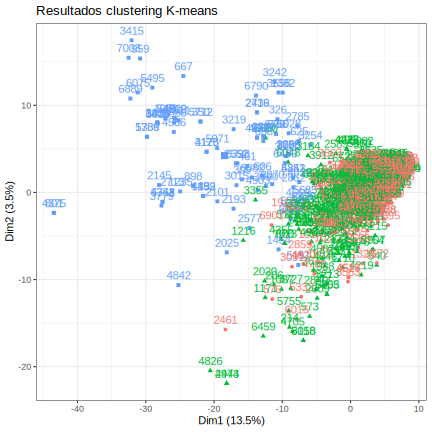
\includegraphics[width=\textwidth]{IMG/R2.jpg}
		\caption{Rotación de la imagen.}
		\label{fig:f8}
	\end{minipage}\hfill
\end{figure}

Tras aplicar una rotación de 30 grados respecto al inicio de la imagen, que es el pixel superior izquierdo, se muestra como gran parte de la imagen original sale del cuadro, esto debido a que la transformación hace el mapeo con la rotación y muestra unicamente lo que debería quedar dentro de la imagen.

\newpage

\section{Resultados de aplicar escalado no uniforme}

\begin{figure}[h!]
	\centering
	\begin{minipage}{0.8\textwidth}
		\centering
		\includegraphics[width=\textwidth]{IMG/R3.jpg}
		\caption{Escalado no uniforme de la imagen.}
		\label{fig:f9}
	\end{minipage}\hfill
\end{figure}

Tras aplicar un escalado no uniforme a la imagen de 1.5 en $X$ y de 0.5 en $Y$, se observa de forma muy marcada como a lo ancho de la imagen, cabe en la mitad del espacio de la imagen original sin mayor problema, pero a lo largo se muestra como la imagen se "desborda" de la pantalla.

\newpage

\section{Resultados de aplicar todo}

\begin{figure}[h!]
	\centering
	\begin{minipage}{0.8\textwidth}
		\centering
		\includegraphics[width=\textwidth]{IMG/R4.jpg}
		\caption{Traslación, rotación y escalado de la imagen.}
		\label{fig:f10}
	\end{minipage}\hfill
\end{figure}

Se muestra el resultado de aplicar una traslación de -40 unidades en $X$, 60 unidades en $Y$, un escalado de 0.8 y 1.2 respectivamente junto con una rotación de -30 grados. El resultado de todo esto es la imagen rotada tal que se ve de forma diagonal y se puede decir que "estirada" por el escalamiento.

\newpage

\section{Resultados de todas las pruebas}

\begin{figure}[h!]
	\centering
	\begin{subfigure}[b]{0.45\textwidth}
		\includegraphics[width=\textwidth]{IMG/R1.jpg}
		\caption{Traslación de la imagen}
		\label{fig:r1}
	\end{subfigure}\hfill
	\begin{subfigure}[b]{0.45\textwidth}
		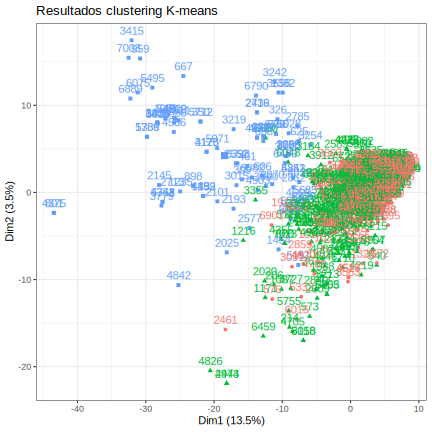
\includegraphics[width=\textwidth]{IMG/R2.jpg}
		\caption{Rotación de la imagen}
		\label{fig:r2}
	\end{subfigure}
	\vspace{\baselineskip} % Espacio vertical entre filas
	\begin{subfigure}[b]{0.45\textwidth}
		\includegraphics[width=\textwidth]{IMG/R3.jpg}
		\caption{Escalado no uniforme de la imagen}
		\label{fig:r3}
	\end{subfigure}\hfill
	\begin{subfigure}[b]{0.45\textwidth}
		\includegraphics[width=\textwidth]{IMG/R4.jpg}
		\caption{Traslación, rotación y escalado de la imagen.}
		\label{fig:r4}
	\end{subfigure}
	\caption{Resumen de los resultados}
	\label{fig:cuadro_r}
\end{figure}




\newpage
	
\section{Conclusiones}
	
Tras la implementación y los experimentos realizados con las transformaciones afines, se observa que cumple bastante bien su trabajo de aplicar las transformaciones sobre la imagen original para proyectarla y luego representarla sobre su espacio original. Lo destacable aquí es que la imagen utilizada al no tener alguna rotación o re escalado por si misma no permite poner en practica que tan buena seria la transformación en el caso de tratar de restaurar la imagen a su estado original. Es decir, partir de una imagen como la mostrada en el resultado de aplicar todas las transformaciones o en donde se aplica el escalado uniforme y tratar de dejarla como se ve la imagen base.
\newpage

	
\section{Referencias}  % Sección numerada de referencias
\bibliographystyle{apalike}  % Estilo de citas (puedes cambiarlo)
\bibliography{Biblio}        % Nombre del archivo BibTeX (sin extensión)

\newpage
	
\section{Anexos}	
\subsection{Implementación de las transformaciones afines con la interpolación bilineal}
\begin{minted}[linenos,firstnumber=1]{matlab}

%% Interpolación bilineal %%
function valor = bilineal(imagen,x,y)
[filas,columnas] = size(imagen);

% Coordenadas vecinas más próximas
x1 = floor(x); x2 = ceil(x);
y1 = floor(y); y2 = ceil(y);

% Limitar los valores al rango válido
if x1 < 1 || x2 > columnas || y1 < 1 || y2 > filas
valor = 0;
return;
end

% Valores de píxeles vecinos
Q11 = double(imagen(y1,x1));
Q21 = double(imagen(y1,x2));
Q12 = double(imagen(y2,x1));
Q22 = double(imagen(y2,x2));

% Pesos
dx = x - x1;
dy = y - y1;

% Interpolación bilineal
valor = (1-dx)*(1-dy)*Q11 + ...
dx*(1-dy)*Q21 + ...
(1-dx)*dy*Q12 + ...
dx*dy*Q22;
end

%% Transformación afin %%
function salida = trans_afin(imagen,Tx,Ty,sx,sy,theta)
% Definir una matriz de escalado %%
S = [sx, 0, 0;
0, sy, 0;
0, 0, 1];
% Definir una matriz de rotación en grados (no radianes) %%
% Convertir los grados a radianes
theta1 = theta * pi/180;
% Definir la matriz de rotación %
R = [cos(theta1), -sin(theta1),0;
sin(theta1), cos(theta1), 0;
0,0,1];
% Definir la matriz de Traslación %%
T = [1,0,Tx;
0, 1, Ty;
0, 0, 1];
% Orden de aplicación %%
% Se define el orden de aplicación tal cual se desarrollaron: Escalar,
% Rotar y Trasladar en ese orden.   
M = T * R * S;
% Base de la salida %%
D = size(imagen);
salida = zeros(D,"uint8");
% Inversa de la matriz de transformación% 
Minv = inv(M);
% Aplicar aqui la interpolación %
for i = 1:D(1)
for j = 1:D(2)
% Coordenadas de destino (x', y')
destino = [j;i;1];

% Coodenadas de origen (x,y) con la inversa %
origen = Minv * destino;
x = origen(1);
y = origen(2);
% Verificar validez del rango
if x>=1 && x<=D(2) && y>=1 && y<=D(1)
%  Aplicar la interpolación
valor = bilineal(imagen,x,y);
salida(i,j) = uint8(valor);
end
end
end
end


%% Prueba de la transformación %%
I = imread("IMG\\F1.jpg");
imagen = rgb2gray(I);
%% Mostrar la imagen %
imshow(imagen);

%% Solo traslación %
R1 = trans_afin(imagen,50,30,1,1,0);
imshow(R1)
%% Solo rotación %
R2 = trans_afin(imagen,0,0,1,1,30);
imshow(R2)
%% Escalado NO uniforme %
R3 = trans_afin(imagen,0,0,1.5,0.5,0);
imshow(R3)
%% Combinación completa %
R4 = trans_afin(imagen,-40,60,0.8,1.2,-30);
imshow(R4)

\end{minted}
	
	
	
	
\end{document}

